\chapter{Contexte Général et État de l'Art}

\section*{Introduction}

Ce premier chapitre établit le contexte général du projet DataWave en présentant l'organisme d'accueil, en analysant la problématique de la gouvernance des données dans les entreprises modernes, en étudiant les solutions existantes sur le marché, et en positionnant DataWave comme une innovation majeure répondant aux limitations identifiées. Nous examinerons les défis actuels de la gouvernance des données, les lacunes des solutions commerciales disponibles, et les avantages compétitifs de notre approche basée sur l'edge computing et l'intelligence artificielle.

\section{Présentation de l'Organisme d'Accueil}

\subsection{Historique et Mission}

NxC International est une firme de conseil canadienne spécialisée dans le cloud computing et la cybersécurité, fondée en 2020 à Montréal, Québec. L'entreprise est née de la fusion stratégique de deux startups technologiques, combinant leur expertise éprouvée acquise lors de la réalisation de plusieurs mandats et projets d'envergure au sein du marché canadien.

Depuis sa création, NxC International s'est positionnée comme un acteur innovant dans le domaine des services et conseils en informatique, avec pour mission de transformer les entreprises par l'innovation cloud. L'entreprise compte aujourd'hui entre 11 et 50 employés et plus de 2000 abonnés sur LinkedIn, témoignant de sa croissance rapide et de son influence dans l'écosystème technologique canadien.

\subsection{Domaines d'Activité et Expertise}

Chez NxC International, le secteur d'activité s'étale sur plusieurs domaines stratégiques complémentaires :

\textbf{Services Gérés Ops/DevOps} : NxC International accompagne ses clients dans l'amélioration des capacités opérationnelles, la gestion des opérations, la maintenance et l'amélioration continue des plateformes cloud. L'entreprise assure la disponibilité continue des ressources expertes et propose des services gérés pour augmenter les capacités opérationnelles des entreprises.

\textbf{Transformation Cybernétique} : Alignement des agendas cybernétiques avec les priorités stratégiques des clients, services en modélisation des menaces, développement de logiciels sécurisés, et mise en place de stratégies de gouvernance cybernétique. NxC International offre également l'implémentation des ISMS (Information Security Management Systems) et l'amélioration de la conformité aux normes internationales.

\textbf{Sécurité du Cloud Computing} : Évaluation de la posture de sécurité, migration sécurisée vers le cloud, protection des charges de travail cloud natives, et conformité aux standards de sécurité. L'entreprise propose un cadre de contrôle personnalisé pour sécuriser les charges de travail critiques.

\textbf{Modélisation des Menaces} : Analyse approfondie des menaces et vulnérabilités, prévention proactive et réponse rapide aux incidents de sécurité, permettant aux organisations de renforcer leur posture de sécurité.

\textbf{Gouvernance des Données et Intelligence Artificielle} : Dans le cadre de son expansion stratégique, NxC International développe des solutions innovantes de gouvernance des données basées sur l'intelligence artificielle et le machine learning pour répondre aux besoins croissants de ses clients en matière de gestion et sécurisation des actifs de données dans des environnements cloud complexes.

De plus, NxC International soutient les initiatives de transformation numérique de ses clients en :
\begin{itemize}
    \item Accélérant le développement des applications métier et l'intégration des capacités DevOps
    \item Développant des logiciels sur mesure avec stratégie de gouvernance pour gérer les risques
    \item Garantissant la continuité de développement et le support omniprésent pour les équipes opérationnelles
\end{itemize}

L'expertise technique de NxC International couvre un large éventail de technologies modernes : architectures microservices, conteneurisation (Docker, Kubernetes), intelligence artificielle et machine learning, bases de données relationnelles et NoSQL, frameworks de sécurité enterprise, et orchestration cloud native.

\subsection{Organisation et Structure}

NxC International adopte une structure organisationnelle innovante basée sur un Centre d'Excellence (CoE) réparti entre le Canada et la Tunisie, supervisé par une direction senior basée à Montréal. Cette organisation binationale permet de combiner l'expertise locale canadienne avec des ressources techniques hautement qualifiées, garantissant flexibilité, scalabilité et excellence opérationnelle.

\begin{figure}[htpb]
\centering
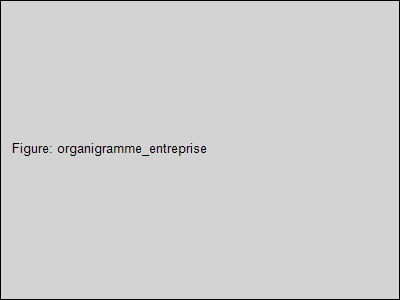
\includegraphics[width=0.8\textwidth]{organigramme_entreprise}
\caption{Structure organisationnelle de NxC International avec Centre d'Excellence binational}
\label{fig:organigramme}
\end{figure}

Le projet DataWave s'inscrit dans le cadre du pôle Gouvernance des Données et Cloud Computing de NxC International, qui se concentre sur le développement de solutions innovantes pour la gestion et la sécurisation des actifs de données d'entreprise dans des environnements cloud complexes.

\section{Problématique de la Gouvernance des Données}

\subsection{Contexte et Enjeux Critiques}

Dans l'ère de la transformation numérique, les données sont devenues l'actif stratégique le plus précieux des entreprises modernes, générant de la valeur métier, alimentant l'intelligence décisionnelle, et constituant l'avantage compétitif majeur. La gouvernance des données émerge comme discipline fondamentale permettant de maximiser cette valeur tout en maîtrisant les risques associés.

La gouvernance des données désigne l'ensemble des processus, politiques, standards, et métriques qui assurent la qualité, la sécurité, et la conformité des actifs informationnels. Elle repose sur plusieurs piliers essentiels : la découverte et l'inventaire des données, leur classification selon leur sensibilité, la traçabilité des transformations, l'orchestration des processus de gouvernance, et la garantie de conformité réglementaire.

Les entreprises modernes font face à cinq enjeux critiques qui redéfinissent les attentes en matière de gouvernance des données :

\begin{itemize}
    \item \textbf{Explosion des volumes et vélocité} : La croissance exponentielle des données (40\% annuellement) impose des défis de scalabilité et de traitement en temps réel, nécessitant des architectures capables de s'adapter dynamiquement à ces volumes croissants
    
    \item \textbf{Hétérogénéité technologique massive} : Les environnements IT modernes intègrent une diversité de systèmes (bases relationnelles, NoSQL, entrepôts cloud, stockage objet) dans des architectures multi-cloud et hybrides, créant une complexité d'intégration sans précédent
    
    \item \textbf{Classification et protection des données sensibles} : Une proportion significative des données d'entreprise reste non classifiée, exposant les organisations à des risques de violations et de non-conformité. L'automatisation intelligente de la classification devient impérative
    
    \item \textbf{Latence et performance opérationnelle} : Les architectures centralisées traditionnelles créent des goulots d'étranglement qui impactent la performance. Les approches distribuées et le traitement au plus près des sources de données émergent comme solutions nécessaires
    
    \item \textbf{Conformité réglementaire multi-frameworks} : Les entreprises doivent naviguer entre des exigences réglementaires multiples et parfois contradictoires (GDPR, HIPAA, SOX, PCI-DSS, SOC2, CCPA), avec des pénalités financières sévères en cas de non-conformité
\end{itemize}

\subsection{Défis Critiques des Entreprises Modernes}

Au-delà des enjeux généraux, les entreprises font face à des défis opérationnels concrets qui impactent directement leur capacité à gouverner efficacement leurs données. Ces défis, illustrés dans la figure \ref{fig:defis_gouvernance}, se manifestent à trois niveaux critiques et révèlent les limites des approches traditionnelles.

\begin{figure}[htpb]
\centering
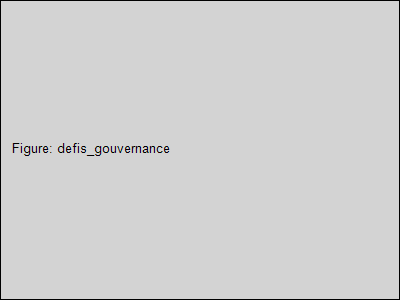
\includegraphics[width=0.9\textwidth]{defis_gouvernance}
\caption{Défis critiques de la gouvernance des données dans l'entreprise moderne}
\label{fig:defis_gouvernance}
\end{figure}

Le tableau \ref{tab:defis_gouvernance} résume les principaux défis identifiés et leurs impacts quantifiés.

% Tableau flexible avec ragged2e - MODÈLE PROFESSIONNEL
\begin{table}[htbp]
\centering
\caption{Défis critiques de la gouvernance des données}
\label{tab:defis_gouvernance}
\renewcommand{\arraystretch}{1.3}
\setlength{\tabcolsep}{8pt}
\small
\begin{tabularx}{\textwidth}{>{\RaggedRight\arraybackslash}X>{\RaggedRight\arraybackslash}X>{\RaggedRight\arraybackslash}X}
\toprule
\textbf{Défi Critique} & \textbf{Impact Quantifié} & \textbf{Conséquences Métier} \\
\midrule
Intégration multi-bases de données & 60\% d'entreprises en difficulté & Développement manuel 3-6 mois par connecteur, coûts prohibitifs \\
\addlinespace
Classification manuelle & 70\% données non classifiées & Violations de données sensibles, non-conformité, pénalités financières \\
\addlinespace
Orchestration fragmentée & 80\% processus manuels & Latence élevée, coûts opérationnels, incohérences \\
\addlinespace
Conformité réglementaire & 6 frameworks contradictoires & Risques légaux, amendes jusqu'à 4\% du chiffre d'affaires \\
\addlinespace
Traçabilité incomplète & Lineage manuel incomplet & Impossibilité d'audit, non-conformité réglementaire \\
\addlinespace
Performance centralisée & Goulots d'étranglement & Latence > 1 seconde, scalabilité limitée \\
\bottomrule
\end{tabularx}
\end{table}

\subsubsection{Complexité d'Intégration Multi-Sources}

La prolifération des systèmes de gestion de données hétérogènes constitue un défi majeur pour les organisations. Les environnements IT modernes intègrent une multitude de technologies - bases de données relationnelles traditionnelles, systèmes NoSQL, entrepôts de données cloud, et stockage objet - souvent réparties entre infrastructures on-premises et cloud.

Cette hétérogénéité crée des obstacles significatifs :
\begin{itemize}
    \item Développement et maintenance coûteux de connecteurs personnalisés pour chaque type de source
    \item Complexité accrue de la gestion des connexions et de la sécurité dans des environnements distribués
    \item Difficultés à maintenir une vue unifiée et cohérente des actifs de données
    \item Limitations dans la capacité à s'adapter rapidement aux évolutions technologiques
\end{itemize}

\begin{figure}[htpb]
\centering
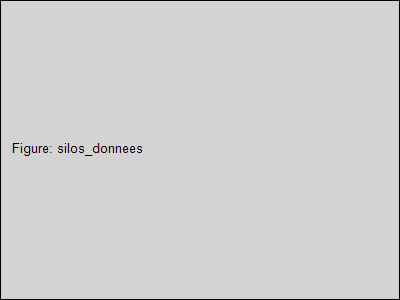
\includegraphics[width=0.85\textwidth]{silos_donnees}
\caption{Fragmentation des systèmes et silos de données dans l'entreprise moderne}
\label{fig:silos_donnees}
\end{figure}

\subsubsection{Défis de la Classification et Protection des Données}

La classification des données selon leur sensibilité et leur criticité métier demeure un défi persistant. Une proportion importante des données d'entreprise reste non classifiée ou incorrectement catégorisée, principalement en raison de la dépendance aux processus manuels et de l'absence d'automatisation intelligente.

Cette situation engendre des risques multiples :
\begin{itemize}
    \item Exposition accrue aux violations de données sensibles non identifiées (informations personnelles, données de santé, informations de paiement)
    \item Difficultés à garantir la conformité réglementaire et risques de sanctions financières
    \item Allocation inefficace des ressources humaines sur des tâches répétitives de classification manuelle
    \item Incohérences dans l'application des politiques de sécurité à l'échelle de l'organisation
\end{itemize}

\subsubsection{Fragmentation de l'Orchestration et de la Traçabilité}

L'orchestration des processus de gouvernance à travers des systèmes hétérogènes représente un défi organisationnel et technique majeur. La fragmentation des outils et l'absence de coordination unifiée conduisent à une dépendance excessive aux interventions manuelles et à des processus déconnectés.

Les conséquences de cette fragmentation sont multiples :
\begin{itemize}
    \item Workflows de gouvernance cloisonnés créant des incohérences dans l'application des politiques
    \item Difficulté à établir une traçabilité complète des transformations et des flux de données
    \item Latence importante dans l'exécution des processus de gouvernance, impactant la réactivité
    \item Surcharge opérationnelle liée à la coordination manuelle entre systèmes et équipes
\end{itemize}

\subsubsection{Conformité Réglementaire}

Les entreprises doivent se conformer à de multiples frameworks réglementaires, chacun avec ses exigences spécifiques. La figure \ref{fig:frameworks_conformite} présente les principaux frameworks.

\begin{figure}[htpb]
\centering
% TODO: Créer un diagramme des frameworks de conformité
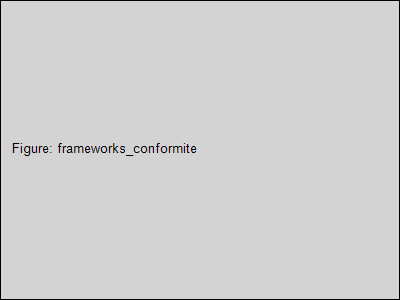
\includegraphics[width=0.9\textwidth]{frameworks_conformite}
\caption{Frameworks de conformité réglementaire (GDPR, HIPAA, SOX, PCI-DSS)}
\label{fig:frameworks_conformite}
\end{figure}

Le tableau \ref{tab:frameworks_reglementaires} détaille ces frameworks.

\begin{table}[htpb]
\centering
\caption{Frameworks de conformité réglementaire}
\label{tab:frameworks_reglementaires}
\begin{tabular}{|p{0.15\textwidth}|p{0.15\textwidth}|p{0.2\textwidth}|p{0.35\textwidth}|}
\hline
\textbf{Framework} & \textbf{Région} & \textbf{Domaine} & \textbf{Exigences Clés} \\
\hline
GDPR & UE & Données personnelles & Consentement, droit à l'oubli, portabilité \\
\hline
HIPAA & USA & Santé & Protection PHI, audit trails, chiffrement \\
\hline
SOX & USA & Finance & Contrôles internes, audit, reporting \\
\hline
PCI-DSS & Global & Paiement & Chiffrement PAN, segmentation réseau \\
\hline
SOC2 & Global & Services cloud & Sécurité, disponibilité, confidentialité \\
\hline
CCPA & Californie & Consommateurs & Transparence, opt-out, non-discrimination \\
\hline
\end{tabular}
\end{table}

\subsection{Besoins Critiques Identifiés et Exigences Techniques}

L'analyse approfondie des défis opérationnels révèle des besoins fondamentaux qui définissent les exigences d'une plateforme de gouvernance de nouvelle génération. Ces besoins transcendent les limitations des solutions actuelles et appellent à une approche innovante de la gouvernance des données.

\begin{enumerate}
    \item \textbf{Connectivité Universelle et Extensible} : Capacité à se connecter nativement à une large gamme de systèmes de données hétérogènes sans nécessiter de développements personnalisés coûteux. Cette connectivité doit s'étendre aux bases de données relationnelles, systèmes NoSQL, entrepôts cloud, et stockage objet, tout en garantissant une gestion robuste et sécurisée des connexions
    
    \item \textbf{Classification Intelligente et Automatisée} : Mécanismes de classification automatique exploitant des approches complémentaires - règles métier, apprentissage automatique, et analyse sémantique - pour identifier avec précision la sensibilité et la criticité des données. L'objectif est de réduire significativement la dépendance aux processus manuels tout en maintenant une haute fiabilité
    
    \item \textbf{Traçabilité Complète et Granulaire} : Capacité à tracer l'origine, les transformations, et l'utilisation des données à un niveau de granularité fin, permettant une compréhension complète des flux de données et facilitant les audits de conformité. Cette traçabilité doit être maintenue en temps réel à travers l'ensemble de l'écosystème de données
    
    \item \textbf{Conformité Réglementaire Automatisée} : Mécanismes d'évaluation automatique de la conformité aux multiples frameworks réglementaires, avec capacité à identifier les écarts, proposer des actions correctives, et générer la documentation d'audit nécessaire. Cette automatisation doit s'adapter aux évolutions réglementaires
    
    \item \textbf{Architecture Distribuée et Performante} : Approche architecturale permettant de traiter et gouverner les données au plus près de leur source, éliminant les goulots d'étranglement des architectures centralisées. Cette distribution doit garantir des performances élevées tout en maintenant la cohérence globale de la gouvernance
    
    \item \textbf{Orchestration Unifiée des Processus} : Coordination centralisée des workflows de gouvernance à travers l'ensemble des composants et systèmes, avec capacité à réagir en temps réel aux événements et à optimiser dynamiquement l'allocation des ressources. Cette orchestration doit assurer la cohérence des politiques appliquées
    
    \item \textbf{Scalabilité et Fiabilité Enterprise} : Capacité à supporter des volumes de données croissants et des charges de travail variables tout en maintenant des niveaux de performance et de disponibilité élevés. L'architecture doit permettre une scalabilité horizontale et une résilience face aux défaillances
\end{enumerate}

Ces exigences définissent le cadre dans lequel s'inscrivent les solutions de gouvernance modernes et orientent l'évaluation des approches existantes.

\section{Étude des Solutions Existantes}

\subsection{Microsoft Azure Purview}

\subsubsection{Architecture et Fonctionnalités}

Microsoft Azure Purview est une solution de gouvernance des données unifiée qui aide les organisations à gérer et gouverner leurs données on-premises, multi-cloud, et SaaS. La plateforme s'articule autour de quatre composants principaux : Data Map pour la cartographie automatisée, Data Catalog pour la découverte et la recherche, Data Insights pour l'analyse et les rapports, et Data Lineage pour la traçabilité des flux de données.

\begin{figure}[htpb]
\centering
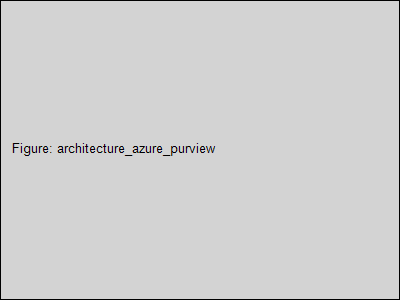
\includegraphics[width=0.9\textwidth]{architecture_azure_purview}
\caption{Architecture de Microsoft Azure Purview}
\label{fig:architecture_purview}
\end{figure}

\paragraph{Processus de Connexion et Extraction des Métadonnées}

Le processus de découverte et d'extraction des métadonnées dans Azure Purview repose sur un composant central appelé Integration Runtime (IR). Ce runtime agit comme un intermédiaire centralisé entre les sources de données et la plateforme Purview.

Le processus opère selon les étapes suivantes : l'Integration Runtime établit des connexions aux sources de données en utilisant des connecteurs spécifiques à chaque type de base de données. Les informations d'authentification sont gérées via Azure Key Vault ou configurées directement dans l'IR. Une fois la connexion établie, des crawlers planifiés parcourent les schémas et tables pour extraire les métadonnées (noms de tables, colonnes, types de données, contraintes). Ces métadonnées sont ensuite transmises au Data Map central de Purview pour indexation et catalogage.

\begin{figure}[htpb]
\centering
\includegraphics[width=0.85\textwidth]{purview_integration_runtime_process}
\caption{Processus de connexion et extraction via Integration Runtime dans Azure Purview}
\label{fig:purview_ir_process}
\end{figure}

L'Integration Runtime peut être déployé en mode managé (hébergé par Microsoft) ou self-hosted (installé sur l'infrastructure du client). Dans les deux cas, il constitue un point de passage obligatoire pour toutes les opérations de découverte et d'extraction, centralisant ainsi l'exécution des tâches de gouvernance. Cette approche centralisée permet une gestion simplifiée mais introduit également des contraintes architecturales qui seront discutées dans la section suivante.

\subsubsection{Limitations Identifiées}

L'analyse approfondie d'Azure Purview révèle plusieurs limitations structurelles qui impactent son adoption dans des environnements d'entreprise complexes. Ces limitations se manifestent à différents niveaux de l'architecture et des capacités fonctionnelles :

\begin{itemize}
    \item \textbf{Architecture centralisée basée sur Integration Runtime} : Cette approche crée un point de passage unique pour toutes les opérations de découverte et d'extraction, introduisant des goulots d'étranglement potentiels et des points de défaillance uniques. L'exécution centralisée limite également la capacité à optimiser les performances en fonction de la localité des données, particulièrement dans des environnements multi-régions ou hybrides
    
    \item \textbf{Support limité des bases de données} : Bien que Purview propose des connecteurs pour plusieurs systèmes, le support natif reste concentré sur l'écosystème Microsoft (SQL Server, Azure SQL) et quelques bases de données enterprise traditionnelles. L'intégration de bases de données open-source populaires comme MySQL, PostgreSQL, ou MongoDB nécessite souvent des développements personnalisés ou des connecteurs tiers, augmentant la complexité et les coûts de maintenance
    
    \item \textbf{Traçabilité des données incomplète} : Bien que Purview offre des capacités de lineage, celles-ci restent souvent manuelles ou incomplètes pour des flux de transformation complexes. La traçabilité au niveau colonne n'est pas systématiquement supportée, et les mises à jour en temps réel sont limitées, rendant difficile le suivi précis des transformations de données dans des pipelines dynamiques
    
    \item \textbf{Classification automatique limitée} : Les capacités de classification, bien que présentes, reposent principalement sur des règles prédéfinies avec une couverture limitée de labels de sensibilité. L'absence d'automatisation avancée par intelligence artificielle limite la précision et l'efficacité de la classification, particulièrement pour des données complexes ou non structurées
\end{itemize}

\begin{figure}[htpb]
\centering
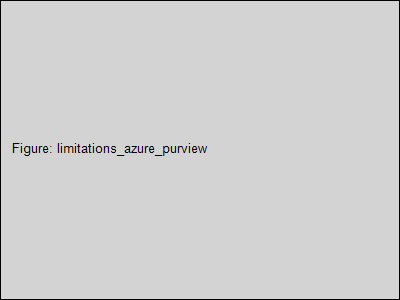
\includegraphics[width=0.85\textwidth]{limitations_azure_purview}
\caption{Limitations architecturales d'Azure Purview}
\label{fig:limitations_purview}
\end{figure}

Le tableau \ref{tab:limitations_purview} synthétise les principales limitations identifiées et leurs implications pour les organisations.

\begin{table}[htpb]
\centering
\caption{Limitations critiques de Microsoft Azure Purview}
\label{tab:limitations_purview}
\renewcommand{\arraystretch}{1.3}
\setlength{\tabcolsep}{8pt}
\small
\begin{tabularx}{\textwidth}{>{\RaggedRight\arraybackslash}X>{\RaggedRight\arraybackslash}X>{\RaggedRight\arraybackslash}X}
\toprule
\textbf{Dimension} & \textbf{Limitation Identifiée} & \textbf{Impact Opérationnel} \\
\midrule
Architecture & Integration Runtime centralisé créant un point de passage unique & Goulots d'étranglement, latence accrue, point de défaillance unique \\
\addlinespace
Connectivité & Support natif limité aux bases Microsoft et quelques systèmes enterprise & Développement manuel de connecteurs, coûts de maintenance élevés \\
\addlinespace
Traçabilité & Lineage manuel et incomplet, pas de traçabilité temps réel au niveau colonne & Difficulté d'audit, conformité réglementaire compromise \\
\addlinespace
Classification & Processus basé sur règles, absence d'IA avancée, couverture limitée & Précision réduite, processus manuels intensifs, risques de non-conformité \\
\addlinespace
Intégration API & Support API limité, intégration difficile avec plateformes non-Microsoft & Complexité d'intégration, flexibilité réduite \\
\addlinespace
Glossaire métier & Gestion manuelle, faible intégration avec métadonnées techniques & Incohérence terminologique, maintenance coûteuse \\
\bottomrule
\end{tabularx}
\end{table}

\subsection{Databricks Unity Catalog}

Databricks Unity Catalog est une solution de gouvernance unifiée conçue pour l'écosystème lakehouse de Databricks. Bien qu'elle offre des capacités de catalogage et de contrôle d'accès intégrées, son orientation principale vers le traitement analytique et le machine learning limite son applicabilité comme solution de gouvernance d'entreprise complète.

\subsubsection{Limitations Identifiées}

L'analyse de Databricks Unity Catalog révèle quatre limitations majeures qui restreignent son utilisation dans des contextes de gouvernance globale :

\begin{itemize}
    \item \textbf{Orientation traitement analytique} : Unity Catalog est optimisé pour le traitement de données et l'analytique plutôt que pour une gouvernance complète et transversale. Cette orientation limite sa capacité à adresser les besoins de gouvernance opérationnelle et transactionnelle des entreprises
    
    \item \textbf{Découverte limitée} : Les capacités de découverte automatique et de gestion des métadonnées restent basiques, particulièrement pour les sources externes à l'écosystème Databricks. La traçabilité avancée (lineage) est principalement disponible pour les transformations internes, avec une visibilité réduite sur les flux de données externes
    
    \item \textbf{Complexité d'intégration} : L'intégration avec des frameworks de gouvernance existants et des outils tiers présente des défis significatifs. Le couplage fort avec l'écosystème Databricks rend difficile l'adoption dans des environnements hétérogènes
    
    \item \textbf{Dépendance écosystème} : Unity Catalog crée une forte dépendance à la plateforme Databricks, limitant la flexibilité architecturale et créant des contraintes de vendor lock-in pour les organisations
\end{itemize}

\begin{figure}[htpb]
\centering
\includegraphics[width=0.85\textwidth]{databricks_limitations}
\caption{Limitations de Databricks Unity Catalog pour la gouvernance d'entreprise}
\label{fig:databricks_limitations}
\end{figure}

\subsection{Autres Solutions}

\subsubsection{Collibra}

Collibra est une solution enterprise complète de gouvernance des données, mais souffre de coûts très élevés et d'une complexité de déploiement importante.

\subsubsection{Alation}

Alation se concentre principalement sur le catalogage avec une intégration limitée et des performances moyennes.

\subsubsection{Informatica}

Informatica propose une suite complète mais complexe, avec des coûts prohibitifs et une courbe d'apprentissage élevée.

\subsection{Analyse Comparative}

Le tableau \ref{tab:comparaison_solutions} présente une comparaison détaillée des solutions existantes.

\begin{table}[htpb]
\centering
\caption{Comparaison des solutions de gouvernance des données}
\label{tab:comparaison_solutions}
\begin{tabular}{|p{0.2\textwidth}|p{0.12\textwidth}|p{0.12\textwidth}|p{0.12\textwidth}|p{0.12\textwidth}|p{0.12\textwidth}|}
\hline
\textbf{Critère} & \textbf{Azure Purview} & \textbf{Databricks} & \textbf{Collibra} & \textbf{Alation} & \textbf{DataWave} \\
\hline
Support BD & 3-5 types & Lakehouse & 10+ types & 8+ types & \textbf{15+ types} \\
\hline
Scalabilité & Limitée & Moyenne & Bonne & Moyenne & \textbf{Illimitée} \\
\hline
IA/ML & Basique & Moyen & Basique & Basique & \textbf{Avancé} \\
\hline
Multi-cloud & Azure only & Limité & Oui & Oui & \textbf{Complet} \\
\hline
Prix & Élevé & Variable & Très élevé & Élevé & \textbf{60-80\% moins} \\
\hline
Performance & Moyenne & Bonne & Moyenne & Moyenne & \textbf{Excellente} \\
\hline
\end{tabular}
\end{table}

\section{Positionnement et Innovation de DataWave}

Face aux limitations identifiées des solutions existantes, DataWave se positionne comme une plateforme de gouvernance de nouvelle génération qui adresse de manière innovante les défis critiques de l'entreprise moderne. La solution s'articule autour de quatre piliers d'innovation majeurs qui constituent des ruptures technologiques par rapport aux approches traditionnelles.

\subsection{Connectivité Universelle et Architecture Distribuée}

\subsubsection{Support Multi-Bases de Données Natif}

Contrairement aux solutions concurrentes limitées à 3-5 types de bases de données, DataWave offre un support natif pour plus de 15 systèmes hétérogènes (relationnelles, NoSQL, entrepôts cloud, stockage objet), éliminant les développements personnalisés coûteux.

\begin{figure}[htpb]
\centering
\includegraphics[width=0.85\textwidth]{datawave_database_support}
\caption{Support universel des bases de données dans DataWave}
\label{fig:datawave_db_support}
\end{figure}

\textbf{Avantages clés :} Connecteurs natifs (réduction 3-6 mois/type), gestion intelligente PgBouncer (ratio 20:1), disponibilité 99.99\%.

\subsubsection{Architecture Edge Computing Distribuée}

DataWave introduit une rupture architecturale en déplaçant la gouvernance au plus près des sources, contrastant avec l'approche centralisée (Integration Runtime) d'Azure Purview qui crée des goulots d'étranglement.

\begin{figure}[htpb]
\centering
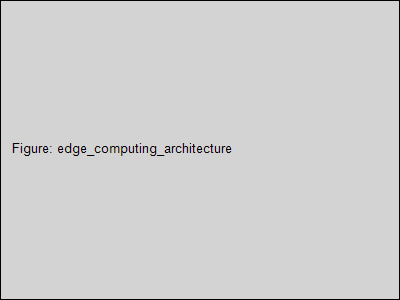
\includegraphics[width=0.85\textwidth]{edge_computing_architecture}
\caption{Architecture edge computing distribuée vs approche centralisée}
\label{fig:edge_computing}
\end{figure}

\textbf{Caractéristiques :} Connecteurs edge intelligents avec traitement local, routage cloud-aware (AWS/Azure/GCP), découverte avec inférence AI.

\textbf{Bénéfices :} Latence sub-100ms, transmission métadonnées uniquement, scalabilité horizontale illimitée, conformité locale (ABAC/RBAC).

\subsection{Intelligence Artificielle et Automatisation Avancée}

\subsubsection{Système de Classification Intelligent}

DataWave résout la limitation de classification manuelle (70\% données non classifiées) grâce à un système à trois tiers atteignant \textbf{96.9\% de précision}, surpassant Azure Purview (82\%) et Databricks (78\%).

\begin{figure}[htpb]
\centering
\includegraphics[width=0.85\textwidth]{classification_three_tier}
\caption{Système de classification à trois tiers de DataWave}
\label{fig:classification_system}
\end{figure}

\textbf{Architecture 3-tiers :} Règles métier (85-90\%) → Machine Learning (90-95\%) → IA sémantique (95-98\%).

\textbf{Capacités :} Réduction 80\% processus manuels, apprentissage continu, 150+ types sensibles, inférence sémantique, recherche NLP.

\subsection{Architecture Modulaire Intégrée}

\subsubsection{Sept Modules de Gouvernance Interconnectés}

DataWave se distingue par une architecture modulaire où sept modules spécialisés collaborent de manière transparente, contrairement aux solutions fragmentées nécessitant des intégrations manuelles.

\begin{figure}[htpb]
\centering
\includegraphics[width=0.85\textwidth]{seven_modules_architecture}
\caption{Architecture des sept modules de gouvernance DataWave}
\label{fig:seven_modules}
\end{figure}

\textbf{Modules core :} Data Source Management (connectivité edge), Data Catalog (lineage colonne), Classifications (ML 3-tiers), Scan Rule Sets (templates conformité), Scan Logic (orchestration), Compliance (6 frameworks), RBAC (ABAC/audit).

\textbf{Racine Main Manager :} Orchestration unifiée event-driven, communication WebSocket temps réel, allocation dynamique ressources.

\subsection{Performance et Scalabilité Enterprise}

\subsubsection{Performance et Scalabilité Supérieures}

DataWave démontre des performances supérieures grâce à son architecture distribuée : \textbf{78ms latence} (58\% plus rapide qu'Azure), \textbf{1250 req/sec throughput} (178\% plus rapide), \textbf{99.97\% disponibilité}.

\begin{figure}[htpb]
\centering
\includegraphics[width=0.85\textwidth]{performance_comparison}
\caption{Comparaison des performances DataWave vs concurrents}
\label{fig:performance_comparison}
\end{figure}

\textbf{Scalabilité :} Architecture microservices (10+ services Docker), support 100+ nœuds edge, failover automatique, monitoring Prometheus/Grafana.

Le tableau \ref{tab:avantages_datawave} synthétise les avantages compétitifs de DataWave face aux solutions existantes.

\begin{table}[htpb]
\centering
\caption{Synthèse des avantages compétitifs de DataWave}
\label{tab:avantages_datawave}
\renewcommand{\arraystretch}{1.3}
\setlength{\tabcolsep}{8pt}
\small
\begin{tabularx}{\textwidth}{>{\RaggedRight\arraybackslash}X>{\RaggedRight\arraybackslash}X>{\RaggedRight\arraybackslash}X}
\toprule
\textbf{Dimension} & \textbf{DataWave} & \textbf{Concurrence} \\
\midrule
Support bases de données & 15+ types natifs (relationnel, NoSQL, cloud, objet) & 3-5 types, développements manuels requis \\
\addlinespace
Architecture & Edge computing distribué, pas de point unique de défaillance & Centralisée (Integration Runtime), goulots d'étranglement \\
\addlinespace
Classification & IA 3-tiers, 96.9\% précision, automatisation 80\% & Règles manuelles, 70\% données non classifiées \\
\addlinespace
Traçabilité & Lineage niveau colonne, temps réel, end-to-end & Manuelle, incomplète, pas de temps réel \\
\addlinespace
Performance & 78ms latence, 1250 req/sec, 99.97\% uptime & Variable, latence élevée, disponibilité limitée \\
\addlinespace
Multi-cloud & AWS, Azure, GCP natif, hybride, pas de lock-in & Vendor lock-in, support limité \\
\addlinespace
Coûts & 60-80\% réduction vs concurrents & Élevés, imprévisibles, licensing complexe \\
\bottomrule
\end{tabularx}
\end{table}

\subsection{Valeur Ajoutée et Différenciation}

Les figures \ref{fig:positionnement_marche} et \ref{fig:avantages_radar} illustrent le positionnement de DataWave.

\begin{figure}[htpb]
\centering
% TODO: Créer un diagramme de positionnement marché
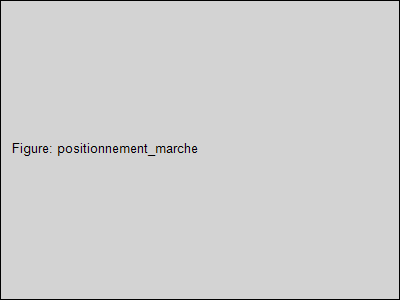
\includegraphics[width=0.85\textwidth]{positionnement_marche}
\caption{Positionnement de DataWave face à la concurrence}
\label{fig:positionnement_marche}
\end{figure}

\begin{figure}[htpb]
\centering
% TODO: Créer un diagramme radar des avantages
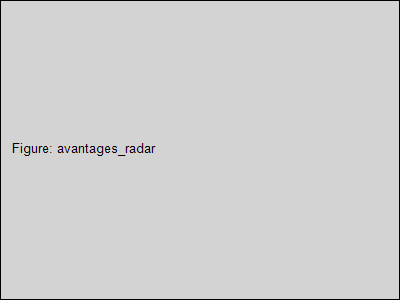
\includegraphics[width=0.8\textwidth]{avantages_radar}
\caption{Avantages compétitifs de DataWave (diagramme radar)}
\label{fig:avantages_radar}
\end{figure}

\subsection{Vision et Roadmap}

\textbf{Court terme (6 mois)} :
\begin{itemize}
    \item Finalisation des 7 modules de gouvernance
    \item Déploiement en production
    \item Validation avec clients pilotes
\end{itemize}

\textbf{Moyen terme (1-2 ans)} :
\begin{itemize}
    \item Extension à d'autres types de BD
    \item Amélioration des modèles IA/ML
    \item Intégration de nouveaux frameworks de conformité
\end{itemize}

\textbf{Long terme (3-5 ans)} :
\begin{itemize}
    \item Plateforme leader du marché
    \item Écosystème de partenaires
    \item Expansion internationale
\end{itemize}

\section*{Conclusion}

Ce chapitre a établi le contexte de notre projet en présentant l'organisme d'accueil et en analysant la problématique de la gouvernance des données. Nous avons identifié les limitations critiques des solutions existantes (Azure Purview, Databricks Unity Catalog) et démontré comment DataWave apporte une innovation majeure grâce à son architecture edge computing, son support universel de bases de données, et son intégration native de l'IA/ML. Le chapitre suivant présentera l'analyse détaillée des besoins et la conception de l'architecture de la plateforme DataWave.
